% Options for packages loaded elsewhere
\PassOptionsToPackage{unicode}{hyperref}
\PassOptionsToPackage{hyphens}{url}
%
\documentclass[
]{book}
\usepackage{amsmath,amssymb}
\usepackage{lmodern}
\usepackage{iftex}
\ifPDFTeX
  \usepackage[T1]{fontenc}
  \usepackage[utf8]{inputenc}
  \usepackage{textcomp} % provide euro and other symbols
\else % if luatex or xetex
  \usepackage{unicode-math}
  \defaultfontfeatures{Scale=MatchLowercase}
  \defaultfontfeatures[\rmfamily]{Ligatures=TeX,Scale=1}
\fi
% Use upquote if available, for straight quotes in verbatim environments
\IfFileExists{upquote.sty}{\usepackage{upquote}}{}
\IfFileExists{microtype.sty}{% use microtype if available
  \usepackage[]{microtype}
  \UseMicrotypeSet[protrusion]{basicmath} % disable protrusion for tt fonts
}{}
\makeatletter
\@ifundefined{KOMAClassName}{% if non-KOMA class
  \IfFileExists{parskip.sty}{%
    \usepackage{parskip}
  }{% else
    \setlength{\parindent}{0pt}
    \setlength{\parskip}{6pt plus 2pt minus 1pt}}
}{% if KOMA class
  \KOMAoptions{parskip=half}}
\makeatother
\usepackage{xcolor}
\IfFileExists{xurl.sty}{\usepackage{xurl}}{} % add URL line breaks if available
\IfFileExists{bookmark.sty}{\usepackage{bookmark}}{\usepackage{hyperref}}
\hypersetup{
  pdftitle={Data reporting in RMarkdown.},
  pdfauthor={Rachael Remington; Anthony Davidson},
  hidelinks,
  pdfcreator={LaTeX via pandoc}}
\urlstyle{same} % disable monospaced font for URLs
\usepackage{color}
\usepackage{fancyvrb}
\newcommand{\VerbBar}{|}
\newcommand{\VERB}{\Verb[commandchars=\\\{\}]}
\DefineVerbatimEnvironment{Highlighting}{Verbatim}{commandchars=\\\{\}}
% Add ',fontsize=\small' for more characters per line
\usepackage{framed}
\definecolor{shadecolor}{RGB}{248,248,248}
\newenvironment{Shaded}{\begin{snugshade}}{\end{snugshade}}
\newcommand{\AlertTok}[1]{\textcolor[rgb]{0.94,0.16,0.16}{#1}}
\newcommand{\AnnotationTok}[1]{\textcolor[rgb]{0.56,0.35,0.01}{\textbf{\textit{#1}}}}
\newcommand{\AttributeTok}[1]{\textcolor[rgb]{0.77,0.63,0.00}{#1}}
\newcommand{\BaseNTok}[1]{\textcolor[rgb]{0.00,0.00,0.81}{#1}}
\newcommand{\BuiltInTok}[1]{#1}
\newcommand{\CharTok}[1]{\textcolor[rgb]{0.31,0.60,0.02}{#1}}
\newcommand{\CommentTok}[1]{\textcolor[rgb]{0.56,0.35,0.01}{\textit{#1}}}
\newcommand{\CommentVarTok}[1]{\textcolor[rgb]{0.56,0.35,0.01}{\textbf{\textit{#1}}}}
\newcommand{\ConstantTok}[1]{\textcolor[rgb]{0.00,0.00,0.00}{#1}}
\newcommand{\ControlFlowTok}[1]{\textcolor[rgb]{0.13,0.29,0.53}{\textbf{#1}}}
\newcommand{\DataTypeTok}[1]{\textcolor[rgb]{0.13,0.29,0.53}{#1}}
\newcommand{\DecValTok}[1]{\textcolor[rgb]{0.00,0.00,0.81}{#1}}
\newcommand{\DocumentationTok}[1]{\textcolor[rgb]{0.56,0.35,0.01}{\textbf{\textit{#1}}}}
\newcommand{\ErrorTok}[1]{\textcolor[rgb]{0.64,0.00,0.00}{\textbf{#1}}}
\newcommand{\ExtensionTok}[1]{#1}
\newcommand{\FloatTok}[1]{\textcolor[rgb]{0.00,0.00,0.81}{#1}}
\newcommand{\FunctionTok}[1]{\textcolor[rgb]{0.00,0.00,0.00}{#1}}
\newcommand{\ImportTok}[1]{#1}
\newcommand{\InformationTok}[1]{\textcolor[rgb]{0.56,0.35,0.01}{\textbf{\textit{#1}}}}
\newcommand{\KeywordTok}[1]{\textcolor[rgb]{0.13,0.29,0.53}{\textbf{#1}}}
\newcommand{\NormalTok}[1]{#1}
\newcommand{\OperatorTok}[1]{\textcolor[rgb]{0.81,0.36,0.00}{\textbf{#1}}}
\newcommand{\OtherTok}[1]{\textcolor[rgb]{0.56,0.35,0.01}{#1}}
\newcommand{\PreprocessorTok}[1]{\textcolor[rgb]{0.56,0.35,0.01}{\textit{#1}}}
\newcommand{\RegionMarkerTok}[1]{#1}
\newcommand{\SpecialCharTok}[1]{\textcolor[rgb]{0.00,0.00,0.00}{#1}}
\newcommand{\SpecialStringTok}[1]{\textcolor[rgb]{0.31,0.60,0.02}{#1}}
\newcommand{\StringTok}[1]{\textcolor[rgb]{0.31,0.60,0.02}{#1}}
\newcommand{\VariableTok}[1]{\textcolor[rgb]{0.00,0.00,0.00}{#1}}
\newcommand{\VerbatimStringTok}[1]{\textcolor[rgb]{0.31,0.60,0.02}{#1}}
\newcommand{\WarningTok}[1]{\textcolor[rgb]{0.56,0.35,0.01}{\textbf{\textit{#1}}}}
\usepackage{longtable,booktabs,array}
\usepackage{calc} % for calculating minipage widths
% Correct order of tables after \paragraph or \subparagraph
\usepackage{etoolbox}
\makeatletter
\patchcmd\longtable{\par}{\if@noskipsec\mbox{}\fi\par}{}{}
\makeatother
% Allow footnotes in longtable head/foot
\IfFileExists{footnotehyper.sty}{\usepackage{footnotehyper}}{\usepackage{footnote}}
\makesavenoteenv{longtable}
\usepackage{graphicx}
\makeatletter
\def\maxwidth{\ifdim\Gin@nat@width>\linewidth\linewidth\else\Gin@nat@width\fi}
\def\maxheight{\ifdim\Gin@nat@height>\textheight\textheight\else\Gin@nat@height\fi}
\makeatother
% Scale images if necessary, so that they will not overflow the page
% margins by default, and it is still possible to overwrite the defaults
% using explicit options in \includegraphics[width, height, ...]{}
\setkeys{Gin}{width=\maxwidth,height=\maxheight,keepaspectratio}
% Set default figure placement to htbp
\makeatletter
\def\fps@figure{htbp}
\makeatother
\setlength{\emergencystretch}{3em} % prevent overfull lines
\providecommand{\tightlist}{%
  \setlength{\itemsep}{0pt}\setlength{\parskip}{0pt}}
\setcounter{secnumdepth}{5}
\usepackage{booktabs}
\ifLuaTeX
  \usepackage{selnolig}  % disable illegal ligatures
\fi
\usepackage[]{natbib}
\bibliographystyle{plainnat}

\title{Data reporting in RMarkdown.}
\usepackage{etoolbox}
\makeatletter
\providecommand{\subtitle}[1]{% add subtitle to \maketitle
  \apptocmd{\@title}{\par {\large #1 \par}}{}{}
}
\makeatother
\subtitle{A quick demo}
\author{Rachael Remington; Anthony Davidson}
\date{2022-05-17}

\begin{document}
\maketitle

{
\setcounter{tocdepth}{1}
\tableofcontents
}
Resources for class 2022 and future 8700 classes

\hypertarget{contents}{%
\chapter{Contents}\label{contents}}

Resources for class 2022 and future 8700 classes

\begin{Shaded}
\begin{Highlighting}[]
\FunctionTok{library}\NormalTok{(tidyverse)}
\end{Highlighting}
\end{Shaded}

\begin{verbatim}
## -- Attaching packages --------------------------------------- tidyverse 1.3.1 --
\end{verbatim}

\begin{verbatim}
## v ggplot2 3.3.5     v purrr   0.3.4
## v tibble  3.1.6     v dplyr   1.0.8
## v tidyr   1.2.0     v stringr 1.4.0
## v readr   2.1.2     v forcats 0.5.1
\end{verbatim}

\begin{verbatim}
## -- Conflicts ------------------------------------------ tidyverse_conflicts() --
## x dplyr::filter() masks stats::filter()
## x dplyr::lag()    masks stats::lag()
\end{verbatim}

\begin{Shaded}
\begin{Highlighting}[]
\FunctionTok{library}\NormalTok{(jtools)}
\end{Highlighting}
\end{Shaded}

\hypertarget{experimental-plan-template}{%
\chapter{Experimental plan template}\label{experimental-plan-template}}

Now that you have been developing a research question over the last few months, the next step is to design a set of experiments that will specifically test your research aims.

We are often focused on the ``cookbook'' aspect of experiments -- the protocols and steps required to conduct each experiment. However, it's critical to spend time designing your overall experimental approach and the finer details to ensure that your research will produce robust data that can be clearly analysed without bias. When we test specific questions, we want to avoid statistical issues such as ``noise'' and ``confounding'' factors.

Terry Neeman will be delivering a workshop to help you strengthen your experimental plan -- both in terms of your proposed design, and to help you more clearly and accurately explain the rationale and set-up of your experiments. This workshop will help you apply the principles taught in BIOL8291 to your own experiment. To prepare, you will create an outline of your experimental plan, focusing on the statistical framework of your design.

Below is an outline of questions for you to answer/justify for each part of your experimental plan. You will also need to draw two figures (digital drawings preferred) for each aim that show:

\begin{enumerate}
\def\labelenumi{\arabic{enumi})}
\item
  a simple overview of the experimental plan related to the research aim,
\item
  a detailed ``snap-shot'' of the experimental set up (i.e., how will the plates, plants, etc. be arranged? Will there be a row-column design? Blocking? Randomization? What treatments will be applied and how many replicates will be tested?)
\end{enumerate}

You can access the template for the experimental plan on Wattle or a copy can be found within this repository. \href{\%22pdfs/3.\%20Statistical\%20Methods\%20in\%20Biology\%20-\%20Chapter\%203.pdf\%22}{DOWNLOAD NOW}.

The template is laid out below as follows:

\hypertarget{research-question}{%
\section{Research Question}\label{research-question}}

\begin{Shaded}
\begin{Highlighting}[]
\CommentTok{\#input question here}
\end{Highlighting}
\end{Shaded}

\hypertarget{experimental-aims}{%
\section{Experimental Aims}\label{experimental-aims}}

For each experiment explain the overall experimental approach (1-3 sentences + overview diagram) list:

\begin{enumerate}
\def\labelenumi{\arabic{enumi})}
\tightlist
\item
  Response/Outcome measure for the experiment;
\item
  The experimental factor(s) of interest;
\item
  The experimental conditions (groups for comparisons);
\item
  The number of replicates/sample size for each condition;
\item
  The experimental control(s);
\item
  Are their any potentially confounding factors (``nuisance factors'')?
\item
  Briefly explain how they will be tracked/or mitigated.
\end{enumerate}

Briefly explain the design of the experiment and provide a diagram that shows a ``snap shot'' of the experimental set-up (e.g., how all the plants under different experimental conditions will be arranged, all the plates in the lab, a flow chart of computational steps, etc.). Make sure to consider and include relevant design aspects like blocking, randomisation, as well as to clearly indicate treatments, replicate numbers, and controls.

\begin{quote}
TIP: Start thinking about how you will analyse your data: ``what statistical tests would you use?''
\end{quote}

\hypertarget{sampling-design}{%
\chapter{Sampling design}\label{sampling-design}}

Outcome vs experimental factors matter and how we contruct models is directly related to the underlying structure of the data we have collected.

\begin{Shaded}
\begin{Highlighting}[]
\CommentTok{\#general packages used}
\FunctionTok{library}\NormalTok{(tidyverse)}
\FunctionTok{library}\NormalTok{(knitr)}
\end{Highlighting}
\end{Shaded}

\hypertarget{terrys-lecture-in-rmarkdown}{%
\section{Terry's lecture in RMarkdown}\label{terrys-lecture-in-rmarkdown}}

Understanding variance is very important for building statistical models. But what it is really about is structuring and generating reproducible experiments.

\begin{Shaded}
\begin{Highlighting}[]
\NormalTok{knitr}\SpecialCharTok{::}\FunctionTok{include\_graphics}\NormalTok{(}\StringTok{"study\_experiment\_design/Experimental{-}plan{-}workshop Terry Neeman 17 May 2002.pdf"}\NormalTok{)}
\end{Highlighting}
\end{Shaded}


\includegraphics{study_experiment_design/Experimental-plan-workshop Terry Neeman 17 May 2002.pdf}

We should all know what these are and how to render a report in RMarkdown. Next we will produce a RMarkdown document for the question we have been working on ready to add data and other sampling design information.

\begin{enumerate}
\def\labelenumi{\arabic{enumi}.}
\tightlist
\item
  Outcome and predictor variables
\item
  Statistical model fitting
\item
  Visual results
\end{enumerate}

\hypertarget{how-would-you-design-your-experiment}{%
\subsection{How would you design your experiment?}\label{how-would-you-design-your-experiment}}

What will the actual design look like? How are the treatments and samples laid out within the experimental layout.

\hypertarget{model-selection}{%
\subsection{Model selection}\label{model-selection}}

\[ null model = lm(activity = 0) \]
More complex model.

\[ model_1 = lm(activity \equiv GBP8 + (1|litter) + (1|mouseID)) \]

\hypertarget{importing-data}{%
\subsection{Importing data}\label{importing-data}}

From the model above it is possible to generate a dataset to produce a model fit and outcomes generated.

\begin{Shaded}
\begin{Highlighting}[]
\FunctionTok{library}\NormalTok{(gridExtra)}
\end{Highlighting}
\end{Shaded}

\begin{verbatim}
## 
## Attaching package: 'gridExtra'
\end{verbatim}

\begin{verbatim}
## The following object is masked from 'package:dplyr':
## 
##     combine
\end{verbatim}

\begin{Shaded}
\begin{Highlighting}[]
\NormalTok{dat }\OtherTok{\textless{}{-}} \FunctionTok{read.csv}\NormalTok{(}\StringTok{"data/Analysis\_ardMods.csv"}\NormalTok{)}
\end{Highlighting}
\end{Shaded}

Select variables from dataset and check the numerical structure is correct in R (numerical, factor etc).

\begin{Shaded}
\begin{Highlighting}[]
\CommentTok{\# 3what response}
\NormalTok{responseACT }\OtherTok{\textless{}{-}} \FunctionTok{c}\NormalTok{(dat}\SpecialCharTok{$}\NormalTok{Delta.Ct.Mean)}
\NormalTok{responseACT2 }\OtherTok{\textless{}{-}} \FunctionTok{c}\NormalTok{(dat}\SpecialCharTok{$}\NormalTok{EQ.Ct.Mean)}


\NormalTok{ p1 }\OtherTok{\textless{}{-}} \FunctionTok{hist}\NormalTok{(responseACT)}
\end{Highlighting}
\end{Shaded}

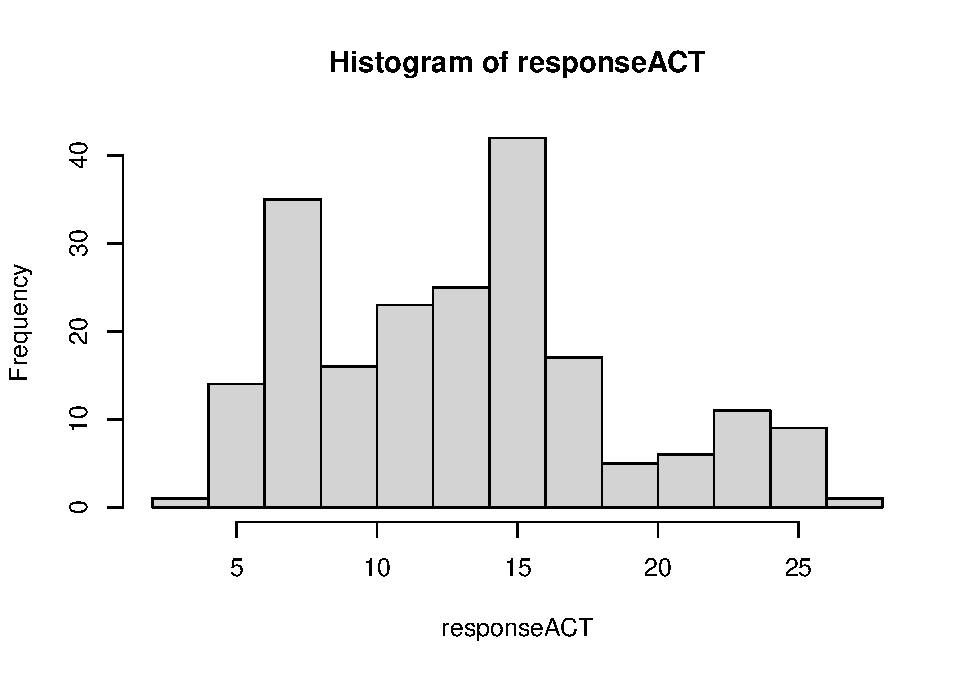
\includegraphics{_main_files/figure-latex/unnamed-chunk-6-1.pdf}

\begin{Shaded}
\begin{Highlighting}[]
\NormalTok{ p2 }\OtherTok{\textless{}{-}} \FunctionTok{hist}\NormalTok{(responseACT2)}
 
 \FunctionTok{par}\NormalTok{(}\AttributeTok{mfrow =} \FunctionTok{c}\NormalTok{(}\DecValTok{2}\NormalTok{,}\DecValTok{2}\NormalTok{))}
 \FunctionTok{hist}\NormalTok{(responseACT2)}
 \FunctionTok{hist}\NormalTok{(responseACT)}
\end{Highlighting}
\end{Shaded}

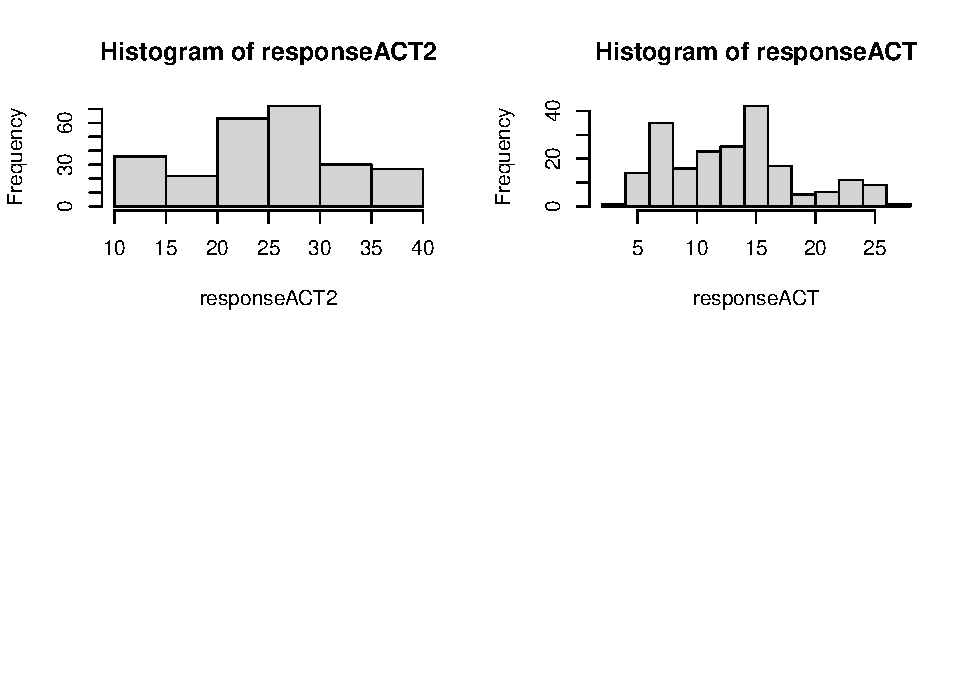
\includegraphics{_main_files/figure-latex/unnamed-chunk-6-2.pdf}

\hypertarget{visualising-data}{%
\subsubsection{Visualising data}\label{visualising-data}}

\hypertarget{reporting}{%
\subsubsection{Reporting}\label{reporting}}

\hypertarget{rmarkdown-reports}{%
\chapter{RMarkdown reports}\label{rmarkdown-reports}}

We should all know what these are and how to render/generate a report or document in RMarkdown.

The next we will produce a RMarkdown document for the question we have been working on ready to add data and other sampling design information.

\begin{Shaded}
\begin{Highlighting}[]
\CommentTok{\#general packages used}
\FunctionTok{library}\NormalTok{(tidyverse)}
\end{Highlighting}
\end{Shaded}

What does this tell us about how RProjects and other funky things work?

\begin{enumerate}
\def\labelenumi{\arabic{enumi}.}
\setcounter{enumi}{2}
\tightlist
\item
  Data import
\end{enumerate}

\begin{Shaded}
\begin{Highlighting}[]
\NormalTok{dat }\OtherTok{\textless{}{-}} \FunctionTok{read.csv}\NormalTok{(}\StringTok{"data/Analysis\_ardMods.csv"}\NormalTok{)}
\FunctionTok{glimpse}\NormalTok{(dat)}
\end{Highlighting}
\end{Shaded}

\begin{verbatim}
## Rows: 380
## Columns: 35
## $ Well                   <chr> "1", "2", "3", "4", "5", "6", "7", "8", "9", "1~
## $ Well.Position          <chr> "A1", "A2", "A3", "A4", "A5", "A6", "A7", "A8",~
## $ Omit                   <chr> "false", "false", "false", "false", "false", "f~
## $ Sample.Name            <chr> "1", "2", "3", "4", "5", "6", "7", "8", "9", "1~
## $ Delta.Ct.SE            <lgl> NA, NA, NA, NA, NA, NA, NA, NA, NA, NA, NA, NA,~
## $ Target.Name            <chr> "Gapdh", "Gapdh", "Gapdh", "Gapdh", "Gapdh", "G~
## $ Task                   <chr> "UNKNOWN", "UNKNOWN", "UNKNOWN", "UNKNOWN", "UN~
## $ Reporter               <chr> "SYBR", "SYBR", "SYBR", "SYBR", "SYBR", "SYBR",~
## $ Quencher               <chr> "None", "None", "None", "None", "None", "None",~
## $ RQ                     <dbl> NA, NA, NA, NA, NA, NA, NA, NA, NA, NA, NA, NA,~
## $ RQ.Min                 <dbl> NA, NA, NA, NA, NA, NA, NA, NA, NA, NA, NA, NA,~
## $ RQ.Max                 <dbl> NA, NA, NA, NA, NA, NA, NA, NA, NA, NA, NA, NA,~
## $ CT                     <chr> "12.909", "14.253", "13.532", "13.377", "14.249~
## $ EQ.Ct.Mean             <dbl> 12.909, 14.253, 13.532, 13.377, 14.249, 15.053,~
## $ EQ.Ct.SE               <lgl> NA, NA, NA, NA, NA, NA, NA, NA, NA, NA, NA, NA,~
## $ Quantity               <lgl> NA, NA, NA, NA, NA, NA, NA, NA, NA, NA, NA, NA,~
## $ Delta.Ct.Mean          <dbl> NA, NA, NA, NA, NA, NA, NA, NA, NA, NA, NA, NA,~
## $ Delta.Delta.Ct         <dbl> NA, NA, NA, NA, NA, NA, NA, NA, NA, NA, NA, NA,~
## $ Automatic.Ct.Threshold <chr> "true", "true", "true", "true", "true", "true",~
## $ Ct.Threshold           <dbl> 0.062, 0.062, 0.062, 0.062, 0.062, 0.062, 0.062~
## $ Automatic.Baseline     <chr> "true", "true", "true", "true", "true", "true",~
## $ Baseline.Start         <int> 3, 3, 3, 3, 3, 3, 3, 3, 3, 3, 3, 3, 3, 3, 3, 3,~
## $ Baseline.End           <int> 9, 11, 10, 10, 11, 13, 10, 10, 11, 10, 9, 9, 10~
## $ Efficiency             <lgl> NA, NA, NA, NA, NA, NA, NA, NA, NA, NA, NA, NA,~
## $ Tm1                    <dbl> 84.395, 84.395, 84.395, 84.395, 84.395, 84.527,~
## $ Comments               <lgl> NA, NA, NA, NA, NA, NA, NA, NA, NA, NA, NA, NA,~
## $ Tm2                    <dbl> NA, NA, NA, NA, NA, NA, NA, NA, NA, NA, NA, NA,~
## $ Amp.Score              <dbl> 1.346, 1.345, 1.352, 1.349, 1.339, 1.356, 1.347~
## $ Tm3                    <dbl> NA, NA, NA, NA, NA, NA, NA, NA, NA, NA, NA, NA,~
## $ Cq.Conf                <dbl> 0.920, 0.872, 0.930, 0.933, 0.974, 0.938, 0.924~
## $ MTP                    <chr> "N", "N", "N", "N", "N", "N", "N", "N", "N", "N~
## $ EXPFAIL                <chr> "N", "N", "N", "N", "N", "N", "N", "N", "N", "N~
## $ NOISE                  <chr> "N", "N", "N", "N", "N", "N", "N", "N", "N", "N~
## $ NOAMP                  <chr> "N", "N", "N", "N", "N", "N", "N", "N", "N", "N~
## $ THOLDFAIL              <chr> "N", "N", "N", "N", "N", "N", "N", "N", "N", "N~
\end{verbatim}

\begin{Shaded}
\begin{Highlighting}[]
\FunctionTok{variable.names}\NormalTok{(dat)}
\end{Highlighting}
\end{Shaded}

\begin{verbatim}
##  [1] "Well"                   "Well.Position"          "Omit"                  
##  [4] "Sample.Name"            "Delta.Ct.SE"            "Target.Name"           
##  [7] "Task"                   "Reporter"               "Quencher"              
## [10] "RQ"                     "RQ.Min"                 "RQ.Max"                
## [13] "CT"                     "EQ.Ct.Mean"             "EQ.Ct.SE"              
## [16] "Quantity"               "Delta.Ct.Mean"          "Delta.Delta.Ct"        
## [19] "Automatic.Ct.Threshold" "Ct.Threshold"           "Automatic.Baseline"    
## [22] "Baseline.Start"         "Baseline.End"           "Efficiency"            
## [25] "Tm1"                    "Comments"               "Tm2"                   
## [28] "Amp.Score"              "Tm3"                    "Cq.Conf"               
## [31] "MTP"                    "EXPFAIL"                "NOISE"                 
## [34] "NOAMP"                  "THOLDFAIL"
\end{verbatim}

\begin{Shaded}
\begin{Highlighting}[]
\FunctionTok{length}\NormalTok{(}\FunctionTok{unique}\NormalTok{(dat}\SpecialCharTok{$}\NormalTok{Well.Position))}
\end{Highlighting}
\end{Shaded}

\begin{verbatim}
## [1] 380
\end{verbatim}

\begin{Shaded}
\begin{Highlighting}[]
\CommentTok{\# outcome \textless{}{-} dat$}

\FunctionTok{table}\NormalTok{(dat}\SpecialCharTok{$}\NormalTok{Omit)}
\end{Highlighting}
\end{Shaded}

\begin{verbatim}
## 
##       false 
##     4   376
\end{verbatim}

\begin{Shaded}
\begin{Highlighting}[]
\NormalTok{removedData }\OtherTok{\textless{}{-}}\NormalTok{ dat }\SpecialCharTok{\%\textgreater{}\%}
  \FunctionTok{filter}\NormalTok{(Omit }\SpecialCharTok{!=} \StringTok{"false"}\NormalTok{)}

\FunctionTok{head}\NormalTok{(removedData)}
\end{Highlighting}
\end{Shaded}

\begin{verbatim}
##                          Well Well.Position Omit Sample.Name Delta.Ct.SE
## 1               Analysis Type    Singleplex                           NA
## 2          Endogenous Control         Gapdh                           NA
## 3 RQ Min/Max Confidence Level          95.0                           NA
## 4            Reference Sample             7                           NA
##   Target.Name Task Reporter Quencher RQ RQ.Min RQ.Max CT EQ.Ct.Mean EQ.Ct.SE
## 1                                    NA     NA     NA            NA       NA
## 2                                    NA     NA     NA            NA       NA
## 3                                    NA     NA     NA            NA       NA
## 4                                    NA     NA     NA            NA       NA
##   Quantity Delta.Ct.Mean Delta.Delta.Ct Automatic.Ct.Threshold Ct.Threshold
## 1       NA            NA             NA                                  NA
## 2       NA            NA             NA                                  NA
## 3       NA            NA             NA                                  NA
## 4       NA            NA             NA                                  NA
##   Automatic.Baseline Baseline.Start Baseline.End Efficiency Tm1 Comments Tm2
## 1                                NA           NA         NA  NA       NA  NA
## 2                                NA           NA         NA  NA       NA  NA
## 3                                NA           NA         NA  NA       NA  NA
## 4                                NA           NA         NA  NA       NA  NA
##   Amp.Score Tm3 Cq.Conf MTP EXPFAIL NOISE NOAMP THOLDFAIL
## 1        NA  NA      NA                                  
## 2        NA  NA      NA                                  
## 3        NA  NA      NA                                  
## 4        NA  NA      NA
\end{verbatim}

\begin{enumerate}
\def\labelenumi{\arabic{enumi}.}
\setcounter{enumi}{3}
\tightlist
\item
  Data visualisation
\end{enumerate}

\begin{Shaded}
\begin{Highlighting}[]
\CommentTok{\# table(dat$Well.Position)}
\FunctionTok{mean}\NormalTok{(dat}\SpecialCharTok{$}\NormalTok{Delta.Ct.Mean, }\AttributeTok{na.rm =} \ConstantTok{TRUE}\NormalTok{)}
\end{Highlighting}
\end{Shaded}

\begin{verbatim}
## [1] 13.08628
\end{verbatim}

\begin{Shaded}
\begin{Highlighting}[]
\FunctionTok{sd}\NormalTok{(dat}\SpecialCharTok{$}\NormalTok{Delta.Ct.Mean, }\AttributeTok{na.rm =} \ConstantTok{TRUE}\NormalTok{)}
\end{Highlighting}
\end{Shaded}

\begin{verbatim}
## [1] 5.507596
\end{verbatim}

\begin{Shaded}
\begin{Highlighting}[]
\FunctionTok{hist}\NormalTok{(dat}\SpecialCharTok{$}\NormalTok{Delta.Ct.Mean)}
\end{Highlighting}
\end{Shaded}

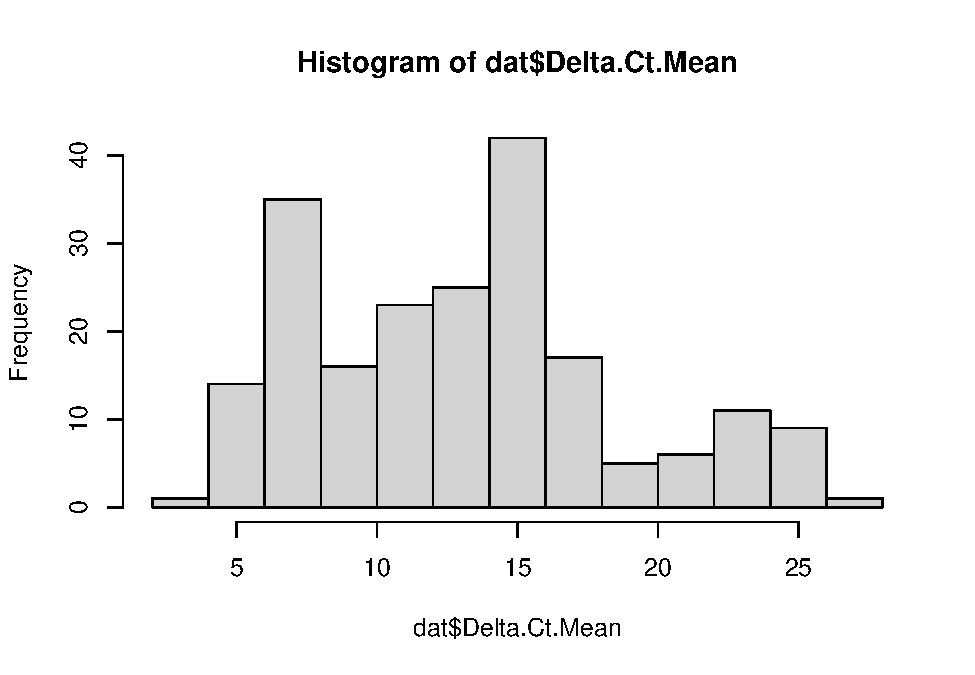
\includegraphics{_main_files/figure-latex/unnamed-chunk-11-1.pdf}

\begin{enumerate}
\def\labelenumi{\arabic{enumi}.}
\setcounter{enumi}{2}
\tightlist
\item
  Data import
\end{enumerate}

\begin{Shaded}
\begin{Highlighting}[]
\NormalTok{dat }\OtherTok{\textless{}{-}} \FunctionTok{read.csv}\NormalTok{(}\StringTok{"data/Analysis\_ardMods.csv"}\NormalTok{)}
\end{Highlighting}
\end{Shaded}

\begin{enumerate}
\def\labelenumi{\arabic{enumi}.}
\setcounter{enumi}{3}
\tightlist
\item
  Data visualisation
\end{enumerate}

\begin{Shaded}
\begin{Highlighting}[]
\CommentTok{\# table(dat$Well.Position)}
\FunctionTok{mean}\NormalTok{(dat}\SpecialCharTok{$}\NormalTok{Delta.Ct.Mean, }\AttributeTok{na.rm =} \ConstantTok{TRUE}\NormalTok{)}
\end{Highlighting}
\end{Shaded}

\begin{verbatim}
## [1] 13.08628
\end{verbatim}

\begin{Shaded}
\begin{Highlighting}[]
\FunctionTok{sd}\NormalTok{(dat}\SpecialCharTok{$}\NormalTok{Delta.Ct.Mean, }\AttributeTok{na.rm =} \ConstantTok{TRUE}\NormalTok{)}
\end{Highlighting}
\end{Shaded}

\begin{verbatim}
## [1] 5.507596
\end{verbatim}

\begin{Shaded}
\begin{Highlighting}[]
\FunctionTok{hist}\NormalTok{(dat}\SpecialCharTok{$}\NormalTok{Delta.Ct.Mean)}
\end{Highlighting}
\end{Shaded}

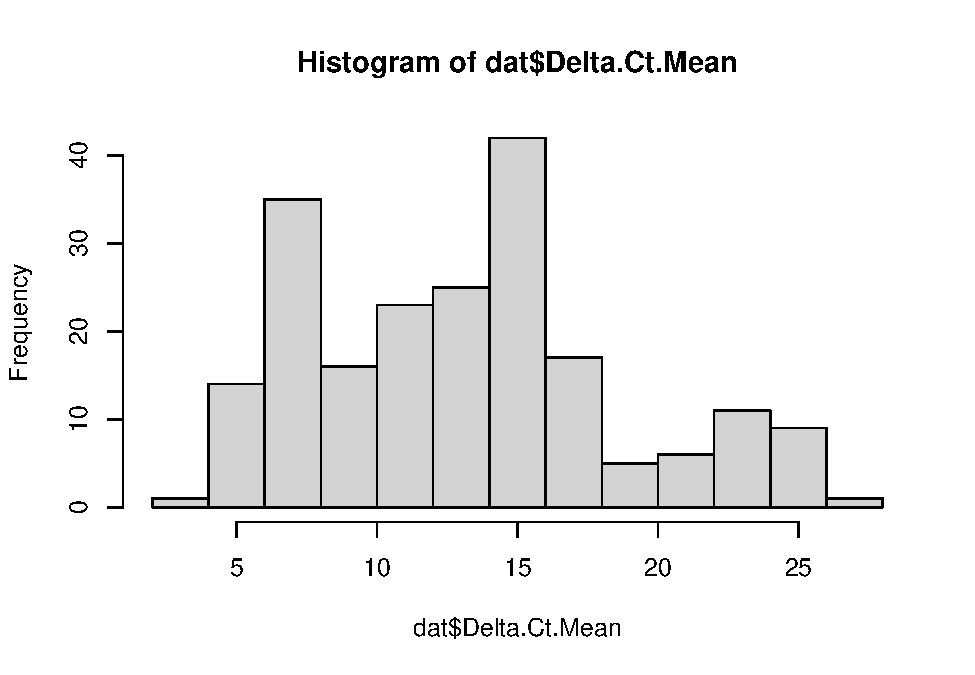
\includegraphics{_main_files/figure-latex/unnamed-chunk-13-1.pdf}

\begin{enumerate}
\def\labelenumi{\arabic{enumi}.}
\setcounter{enumi}{4}
\tightlist
\item
  Tidyverse approach
\end{enumerate}

\begin{Shaded}
\begin{Highlighting}[]
\FunctionTok{variable.names}\NormalTok{(dat)}
\end{Highlighting}
\end{Shaded}

\begin{verbatim}
##  [1] "Well"                   "Well.Position"          "Omit"                  
##  [4] "Sample.Name"            "Delta.Ct.SE"            "Target.Name"           
##  [7] "Task"                   "Reporter"               "Quencher"              
## [10] "RQ"                     "RQ.Min"                 "RQ.Max"                
## [13] "CT"                     "EQ.Ct.Mean"             "EQ.Ct.SE"              
## [16] "Quantity"               "Delta.Ct.Mean"          "Delta.Delta.Ct"        
## [19] "Automatic.Ct.Threshold" "Ct.Threshold"           "Automatic.Baseline"    
## [22] "Baseline.Start"         "Baseline.End"           "Efficiency"            
## [25] "Tm1"                    "Comments"               "Tm2"                   
## [28] "Amp.Score"              "Tm3"                    "Cq.Conf"               
## [31] "MTP"                    "EXPFAIL"                "NOISE"                 
## [34] "NOAMP"                  "THOLDFAIL"
\end{verbatim}

\begin{Shaded}
\begin{Highlighting}[]
\CommentTok{\#sample name}
\CommentTok{\# table(dat$Sample.Name)}
\FunctionTok{table}\NormalTok{(dat}\SpecialCharTok{$}\NormalTok{Target.Name)}
\end{Highlighting}
\end{Shaded}

\begin{verbatim}
## 
##                   16s B Fragilis        Bft      Gapdh   Il-12p40      Il-18 
##          4         47         47         47         47         47         47 
##       Il-6      Il1-b 
##         47         47
\end{verbatim}

\begin{Shaded}
\begin{Highlighting}[]
\FunctionTok{mean}\NormalTok{(}\FunctionTok{as.numeric}\NormalTok{(dat}\SpecialCharTok{$}\NormalTok{CT), }\AttributeTok{na.rm =} \ConstantTok{TRUE}\NormalTok{)}
\end{Highlighting}
\end{Shaded}

\begin{verbatim}
## Warning in mean(as.numeric(dat$CT), na.rm = TRUE): NAs introduced by coercion
\end{verbatim}

\begin{verbatim}
## [1] 24.87021
\end{verbatim}

\begin{Shaded}
\begin{Highlighting}[]
\DocumentationTok{\#\#sumarise over Target Name and find n, mean, mode, median, sd, etc for each of the target names?}
\end{Highlighting}
\end{Shaded}

\begin{enumerate}
\def\labelenumi{\arabic{enumi}.}
\setcounter{enumi}{5}
\item
  Nicer plots using \texttt{ggplot}
\item
  Tidyverse approach
\end{enumerate}

\begin{Shaded}
\begin{Highlighting}[]
\CommentTok{\#tidy data}
\CommentTok{\#tibble}
\end{Highlighting}
\end{Shaded}

\begin{enumerate}
\def\labelenumi{\arabic{enumi}.}
\setcounter{enumi}{5}
\tightlist
\item
  ggplot
\end{enumerate}

Much easier to work this this and tidyverse

\begin{enumerate}
\def\labelenumi{\arabic{enumi}.}
\setcounter{enumi}{6}
\tightlist
\item
  Read a cool sampling design/issue paper
\end{enumerate}

\begin{Shaded}
\begin{Highlighting}[]
\CommentTok{\#general packages used}
\FunctionTok{library}\NormalTok{(tidyverse)}
\end{Highlighting}
\end{Shaded}

We should all know what these are and how to render a report in RMarkdown. Next we will produce a RMarkdown document for the question we have been working on ready to add data and other sampling design information.

\begin{enumerate}
\def\labelenumi{\arabic{enumi}.}
\tightlist
\item
  Outcome and predictor variables
\item
  Other study examples and code
\item
  Other studies with same sampling design
\item
  Other reference material.
\item
  Read a cool sampling design/issue paper
\end{enumerate}

\hypertarget{power-analysis}{%
\chapter{Power analysis}\label{power-analysis}}

Watch this short (ish video) as a summary of what you should understand so far.
What does this tell us about how RProjects and other funky things work?

\begin{Shaded}
\begin{Highlighting}[]
\FunctionTok{library}\NormalTok{(stats)}
\FunctionTok{power.anova.test}\NormalTok{(}\AttributeTok{groups =} \DecValTok{4}\NormalTok{, }\AttributeTok{n =} \DecValTok{5}\NormalTok{, }\AttributeTok{between.var =} \DecValTok{1}\NormalTok{, }\AttributeTok{within.var =} \DecValTok{3}\NormalTok{)}
\end{Highlighting}
\end{Shaded}

\begin{verbatim}
## 
##      Balanced one-way analysis of variance power calculation 
## 
##          groups = 4
##               n = 5
##     between.var = 1
##      within.var = 3
##       sig.level = 0.05
##           power = 0.3535594
## 
## NOTE: n is number in each group
\end{verbatim}

\begin{Shaded}
\begin{Highlighting}[]
\CommentTok{\# Power = 0.3535594}

\FunctionTok{power.anova.test}\NormalTok{(}\AttributeTok{groups =} \DecValTok{4}\NormalTok{, }\AttributeTok{between.var =} \DecValTok{1}\NormalTok{, }\AttributeTok{within.var =} \DecValTok{3}\NormalTok{,}
                 \AttributeTok{power =}\NormalTok{ .}\DecValTok{80}\NormalTok{)}
\end{Highlighting}
\end{Shaded}

\begin{verbatim}
## 
##      Balanced one-way analysis of variance power calculation 
## 
##          groups = 4
##               n = 11.92613
##     between.var = 1
##      within.var = 3
##       sig.level = 0.05
##           power = 0.8
## 
## NOTE: n is number in each group
\end{verbatim}

\begin{Shaded}
\begin{Highlighting}[]
\CommentTok{\# n = 11.92613}

\DocumentationTok{\#\# Assume we have prior knowledge of the group means:}
\NormalTok{groupmeans }\OtherTok{\textless{}{-}} \FunctionTok{c}\NormalTok{(}\DecValTok{120}\NormalTok{, }\DecValTok{130}\NormalTok{, }\DecValTok{140}\NormalTok{, }\DecValTok{150}\NormalTok{)}
\FunctionTok{power.anova.test}\NormalTok{(}\AttributeTok{groups =} \FunctionTok{length}\NormalTok{(groupmeans),}
                 \AttributeTok{between.var =} \FunctionTok{var}\NormalTok{(groupmeans),}
                 \AttributeTok{within.var =} \DecValTok{500}\NormalTok{, }\AttributeTok{power =}\NormalTok{ .}\DecValTok{90}\NormalTok{) }\CommentTok{\# n = 15.18834}
\end{Highlighting}
\end{Shaded}

\begin{verbatim}
## 
##      Balanced one-way analysis of variance power calculation 
## 
##          groups = 4
##               n = 15.18834
##     between.var = 166.6667
##      within.var = 500
##       sig.level = 0.05
##           power = 0.9
## 
## NOTE: n is number in each group
\end{verbatim}

I can not find the additional code from last year but this is a slight variation on the project.

\begin{Shaded}
\begin{Highlighting}[]
\NormalTok{knitr}\SpecialCharTok{::}\FunctionTok{include\_app}\NormalTok{(}\StringTok{"https://mathiasharrer.shinyapps.io/power\_calculator\_meta\_analysis/"}\NormalTok{, }\AttributeTok{height =} \StringTok{"1500px"}\NormalTok{) }
\end{Highlighting}
\end{Shaded}

\begin{verbatim}
## PhantomJS not found. You can install it with webshot::install_phantomjs(). If it is installed, please make sure the phantomjs executable can be found via the PATH variable.
\end{verbatim}

\hypertarget{meta-analysis-power-test}{%
\section{Meta-analysis power test}\label{meta-analysis-power-test}}

\begin{Shaded}
\begin{Highlighting}[]
\CommentTok{\# The included numbers will per calculate power for a meta{-}analysis to detect a summary effect size of 0.2, with an average sample size per group of = 50, a total of 15 effect sizes, and moderate heterogeneity.}

\NormalTok{es }\OtherTok{\textless{}{-}} \FloatTok{0.2} \CommentTok{\# Enter your summary effect size}
\NormalTok{as }\OtherTok{\textless{}{-}} \DecValTok{50}  \CommentTok{\# Average per number per group}
\NormalTok{mk }\OtherTok{\textless{}{-}} \DecValTok{15}  \CommentTok{\# Number of effect sizes}
\NormalTok{hg }\OtherTok{\textless{}{-}} \DecValTok{1}   \CommentTok{\# Heterogeniety (".33" for small, "1" for moderate, \& "3" for large)}

\NormalTok{eq1 }\OtherTok{\textless{}{-}}\NormalTok{ ((as}\SpecialCharTok{+}\NormalTok{as)}\SpecialCharTok{/}\NormalTok{((as)}\SpecialCharTok{*}\NormalTok{(as))) }\SpecialCharTok{+}\NormalTok{ ((es}\SpecialCharTok{\^{}}\DecValTok{2}\NormalTok{)}\SpecialCharTok{/}\NormalTok{(}\DecValTok{2}\SpecialCharTok{*}\NormalTok{(as}\SpecialCharTok{+}\NormalTok{as)))}
\NormalTok{eq2 }\OtherTok{\textless{}{-}}\NormalTok{ hg}\SpecialCharTok{*}\NormalTok{(eq1)}
\NormalTok{eq3 }\OtherTok{\textless{}{-}}\NormalTok{ eq2}\SpecialCharTok{+}\NormalTok{eq1}
\NormalTok{eq4 }\OtherTok{\textless{}{-}}\NormalTok{ eq3}\SpecialCharTok{/}\NormalTok{mk}
\NormalTok{eq5 }\OtherTok{\textless{}{-}}\NormalTok{ (es}\SpecialCharTok{/}\FunctionTok{sqrt}\NormalTok{(eq4))}
\NormalTok{Power }\OtherTok{\textless{}{-}}\NormalTok{ (}\DecValTok{1}\SpecialCharTok{{-}}\FunctionTok{pnorm}\NormalTok{(}\FloatTok{1.96}\SpecialCharTok{{-}}\NormalTok{eq5)) }\CommentTok{\# Two{-}tailed}
\NormalTok{Power}
\end{Highlighting}
\end{Shaded}

\begin{verbatim}
## [1] 0.7798811
\end{verbatim}

\hypertarget{next-steps}{%
\subsubsection{Next steps}\label{next-steps}}

Collect some sample data and application.

z

One aspect that can be challenging when working with RMarkdown documents for manuscripts is references.

The references for a bookdown or rmarkdown file can be included using the following information in the \texttt{yml} header of the index file.

The references for a bookdown or rmarkdown file can be included using the following information in the yml header of the index file.

\begin{verbatim}
\end{verbatim}

\hypertarget{manual-references}{%
\section{Manual references}\label{manual-references}}

\hypertarget{packages}{%
\section{Packages}\label{packages}}

The goal of BIOL877\_setup\_2022 repository here is to provide a starting point for using RMarkdown and RStudio to undertake research.

\hypertarget{download-project-and-files}{%
\section{Download project and files}\label{download-project-and-files}}

We checked and loaded an RMarkdown

This is a \emph{sample} book written in \textbf{Markdown} and extended from the original RMD file. You can use anything that Pandoc's Markdown supports; for example, a math equation \(a^2 + b^2 = c^2\).

\hypertarget{usage}{%
\section{Usage}\label{usage}}

Each \textbf{bookdown} chapter is an .Rmd file, and each .Rmd file can contain one (and only one) chapter. A chapter \emph{must} start with a first-level heading: \texttt{\#\ A\ good\ chapter}, and can contain one (and only one) first-level heading.

Use second-level and higher headings within chapters like: \texttt{\#\#\ A\ short\ section} or \texttt{\#\#\#\ An\ even\ shorter\ section}.

The \texttt{index.Rmd} file is required, and is also your first book chapter. It will be the homepage when you render the book.

\hypertarget{render-book}{%
\section{Render book}\label{render-book}}

You can render the HTML version of this example book without changing anything:

\begin{enumerate}
\def\labelenumi{\arabic{enumi}.}
\item
  Find the \textbf{Build} pane in the RStudio IDE, and
\item
  Click on \textbf{Build Book}, then select your output format, or select ``All formats'' if you'd like to use multiple formats from the same book source files.
\end{enumerate}

Or build the book from the R console:

\begin{Shaded}
\begin{Highlighting}[]
\NormalTok{bookdown}\SpecialCharTok{::}\FunctionTok{render\_book}\NormalTok{()}
\end{Highlighting}
\end{Shaded}

To render this example to PDF as a \texttt{bookdown::pdf\_book}, you'll need to install XeLaTeX. You are recommended to install TinyTeX (which includes XeLaTeX): \url{https://yihui.org/tinytex/}.

\hypertarget{preview-book}{%
\section{Preview book}\label{preview-book}}

As you work, you may start a local server to live preview this HTML book. This preview will update as you edit the book when you save individual .Rmd files. You can start the server in a work session by using the RStudio add-in ``Preview book'', or from the R console:

\begin{Shaded}
\begin{Highlighting}[]
\NormalTok{bookdown}\SpecialCharTok{::}\FunctionTok{serve\_book}\NormalTok{()}
\end{Highlighting}
\end{Shaded}

\hypertarget{output-files}{%
\section{Output files}\label{output-files}}

One of the benefits of working in RMarkdown is that the `gitbook' extension is that it can easily be hosted on github. To do this with the least hurdles is to publish the output files as a github pages site from the \texttt{.docs/}.

  \bibliography{book.bib,packages.bib}

\end{document}
